\documentclass[../thesis.tex]{subfiles}

\begin{document}

%% \section{Related Work}
\section{Contact Forces}
Modeling contacts
\begin{figure}
  \centering
  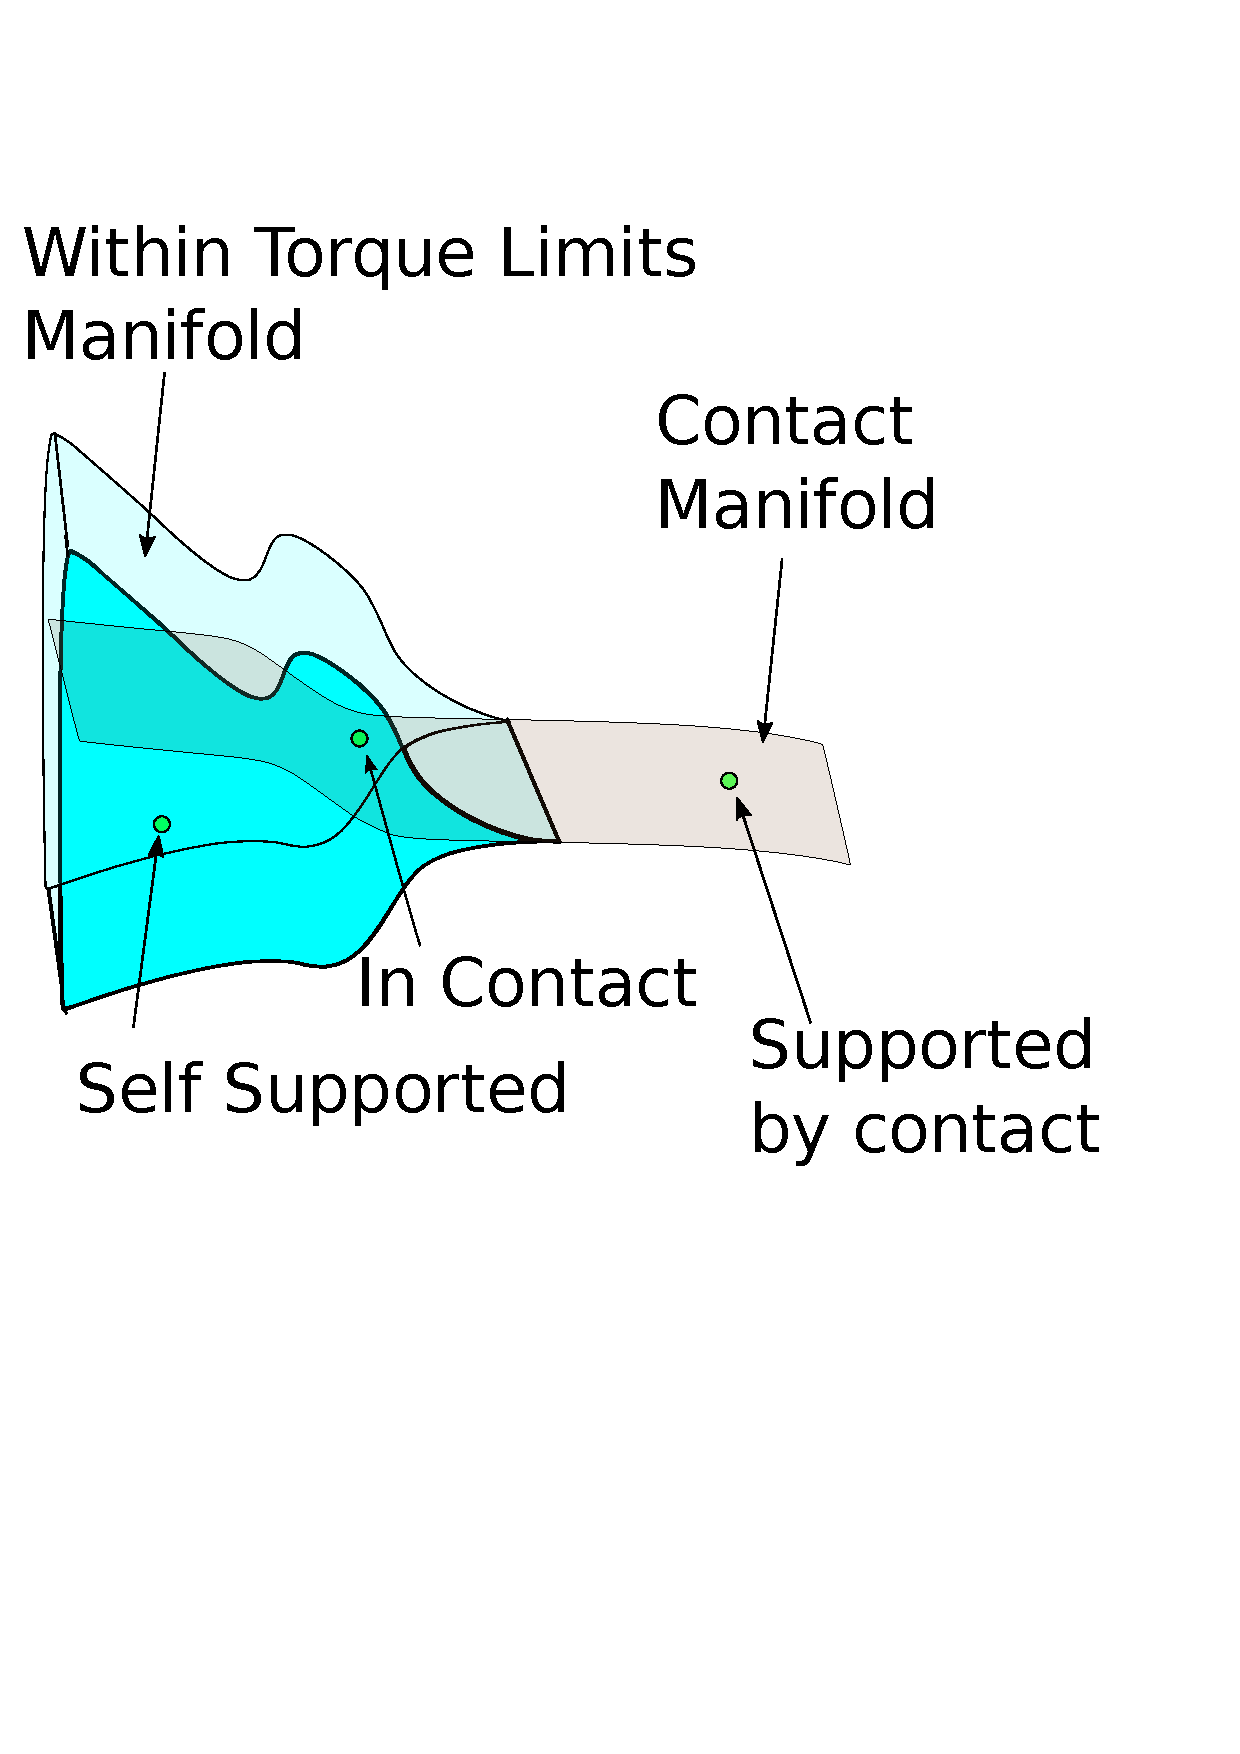
\includegraphics[width=.5\linewidth]{./Planning/thin_manifold.pdf}
  
  \caption{Illustration of valid configuration space for an arm potentially supported by contacts}
  \label{fig:ThinManifold}
\end{figure}


\subsection{Spring Model}
\subsection{}

\section{Bracing}
In path planning for robotic arms any contact with the environment is often considered a collision and thus valid paths have no interaction with the environment.
However environmental contacts can reduce joint torques, damp vibrations, and stabilize an arm.
Despite these benefits contacts are usually avoided because they bring algorithmic complexity during the planning stage and physical danger to the robot and environment if executed improperly.
The increased planning complexity comes from the contact configurations being a measure-zero manifold in the robot configuration space, rendering naive planning in configuration space ineffective. 

The benefits of bracing have been studied since the 1990s.
Lew and Book proposed bracing a micro/macro manipulator with small precise arm mounted on the end of a long course arm and demonstrated bracing of the macro arm against multiple locations of the environment can damp vibration caused by the micro arm \cite{Book1994} \cite{Lew1993}.
Hollis and Hammer explored a similar micro/macro robot design and demonstrated $1 \mu m$ accuracy, well over an order of improvement compared to their unbraced manipulator \cite{Hollis1992}.
Both of these works did not address the planning problem as both contact locations and robot trajectories were manually specified.

Sampling based planners and Trajectory Optimization are two common approaches to path planning, however the measure-zero manifold of contact configurations poses problems to both planning techniques.
Sampling based planners will never sample directly on this manifold, and extending a contact configuration to a new sampled point will immediately leave the contact manifold.
Berenson developed a variation of an RRT planner capable of handling measure-zero manifolds by projecting invalid path extensions onto the valid configuration space \cite{Berenson2009a}.
The method of projection must be provided by the user.


Trajectory Optimization needs a smooth gradient of a cost function and in a naive implementation the benefits of contact will only be realized in a measure-zero domain surrounded by obstacle penetration and no contact regions.
Softening contacts is commonly used in trajectory optimization to produce a gradient for obstacle avoidance, but produces local minima when used for attraction.
Mordatch designed a cost function that continuously models both the benefit and cost of adding contacts and is able to produce trajectories which add and break contacts \cite{Mordatch2012}. 

Rather than solving for a trajectory and contact locations simultaneously some approaches have separated these two problems.
Given a sequence of contact modes for each link, Greenfield computed joint torques to produce desired dynamic behavior and applied this to a climbing snake robot \cite{Greenfield2005}.
Bretl et al. \cite{Bretl2006} developed algorithms for climbing robots that first select contact locations then create collision free trajectories for the robot's limbs between these contact locations.
Tonneau et al \cite{Tonneau} approaches from the opposite direction and first generates a trajectory then considers a discrete set of contacts close to that trajectory.

\section{Discrete Selection of Contact Locations}
\subsection{Walking}
\subsection{Grasping}

\section{Trajectory Optimization}

\begin{figure}
  \centering
  \begin{subfigure}[b]{0.24\linewidth}
    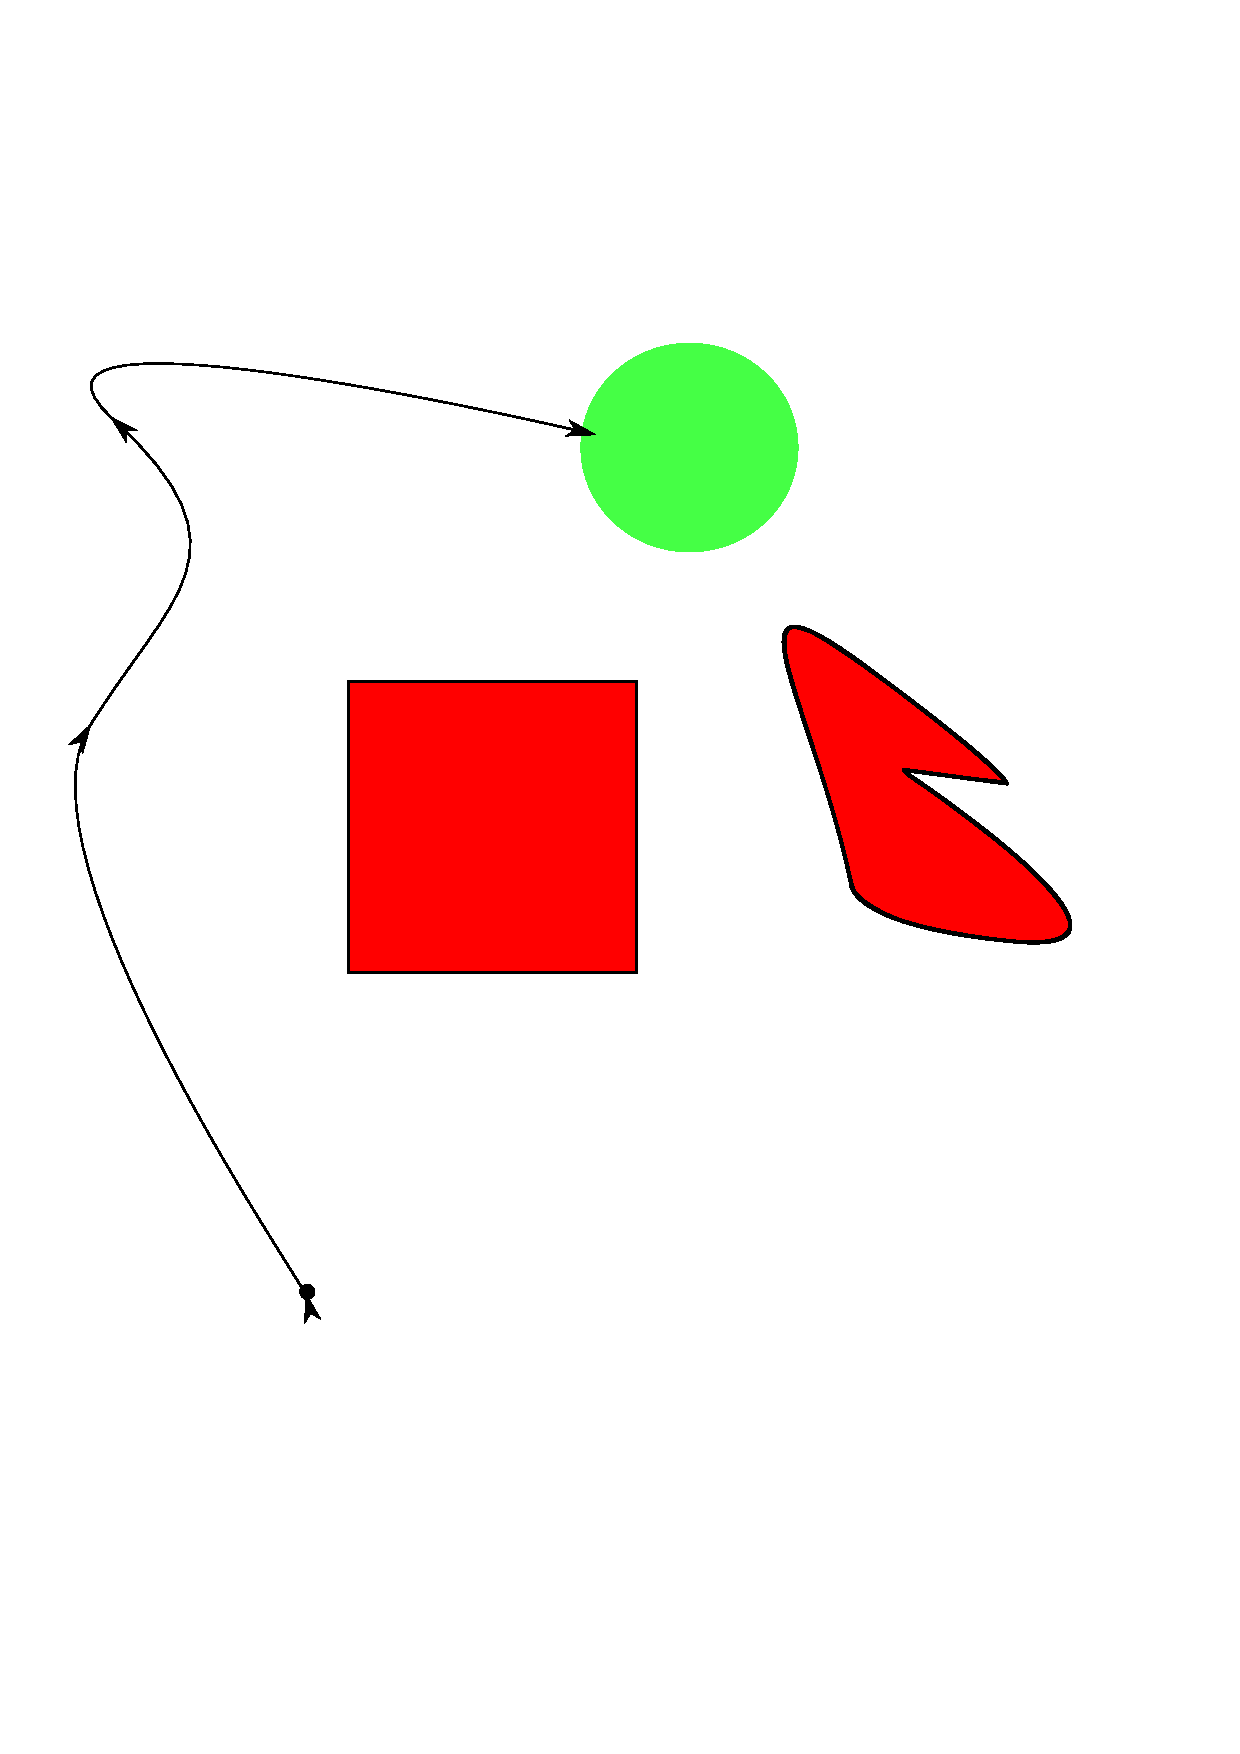
\includegraphics[width=\linewidth]{./Planning/trajectory_1.pdf}
  \end{subfigure}
  \hfill
  \begin{subfigure}[b]{0.24\linewidth}
    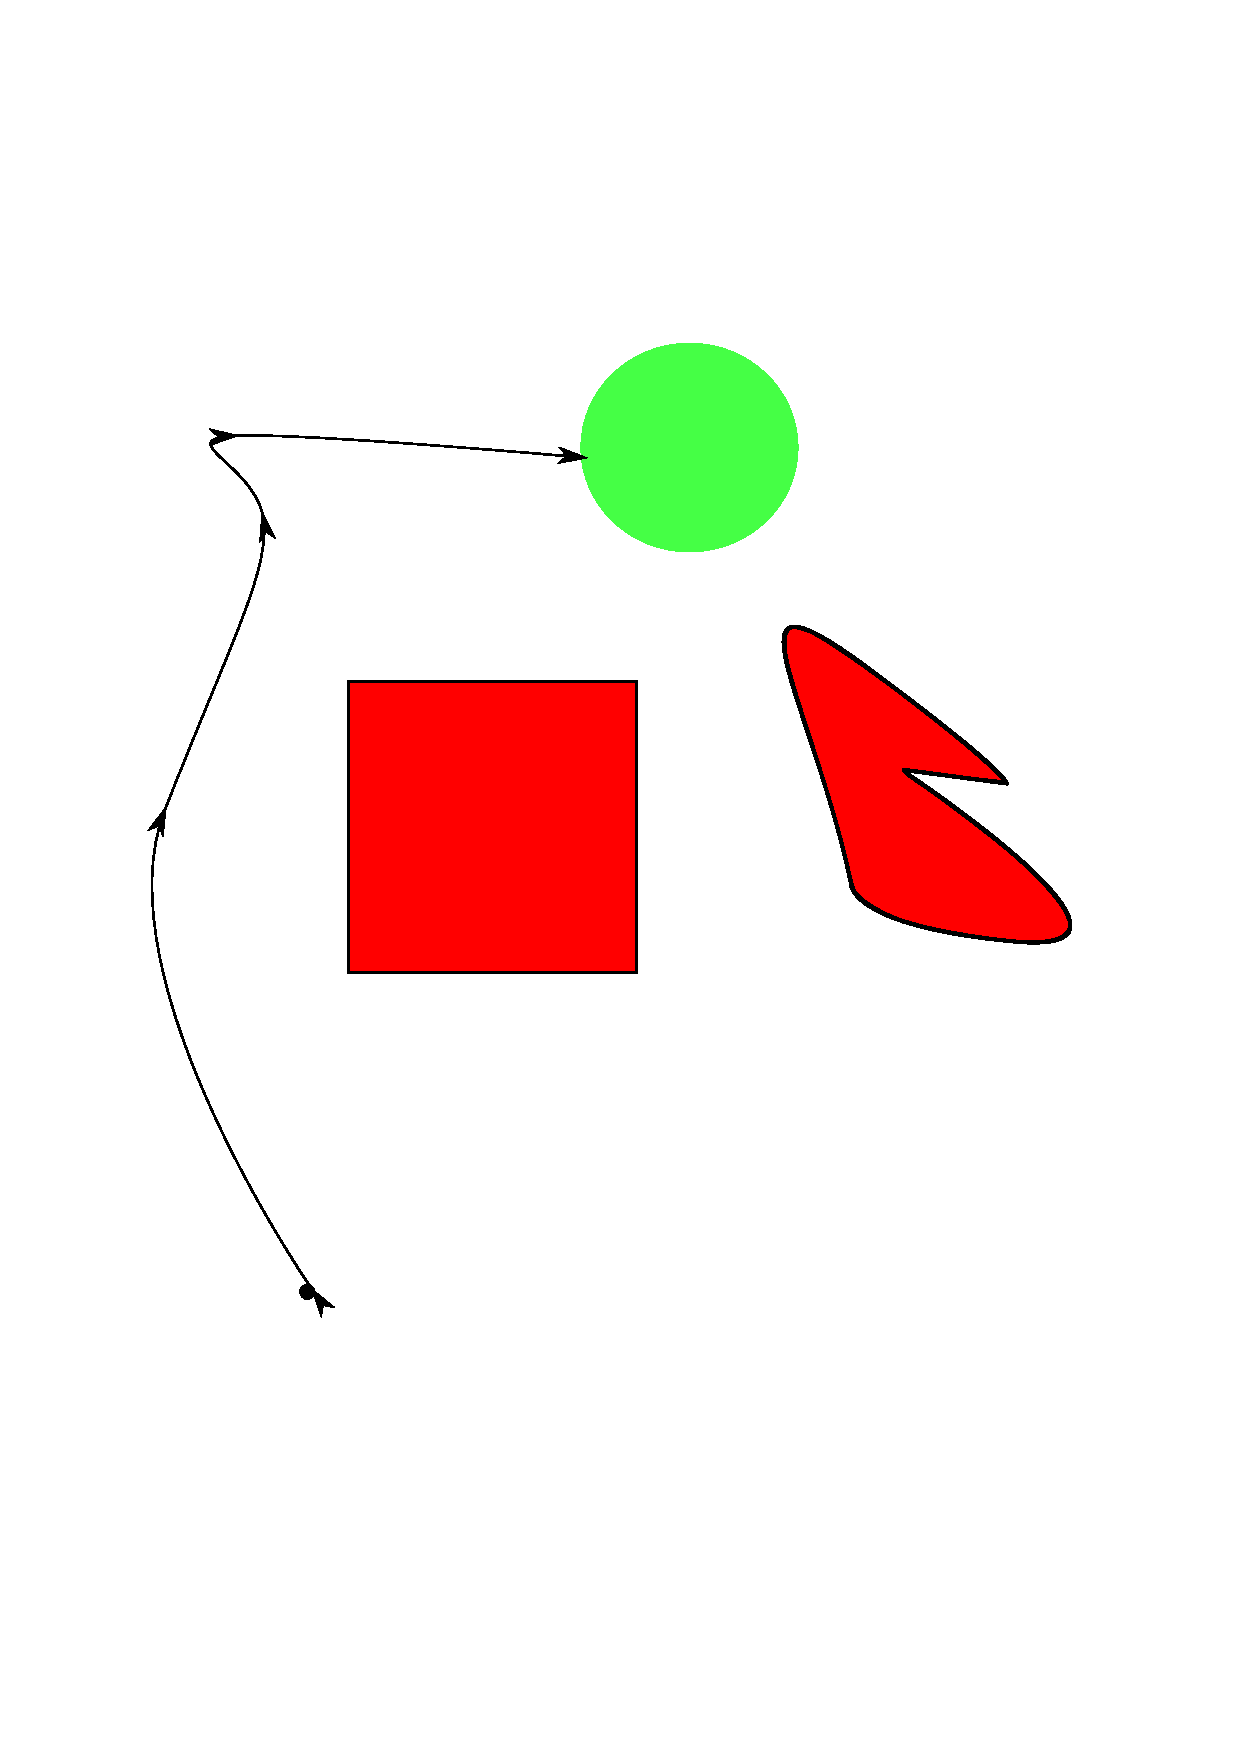
\includegraphics[width=\linewidth]{./Planning/trajectory_2.pdf}    
  \end{subfigure}
  \begin{subfigure}[b]{0.24\linewidth}
    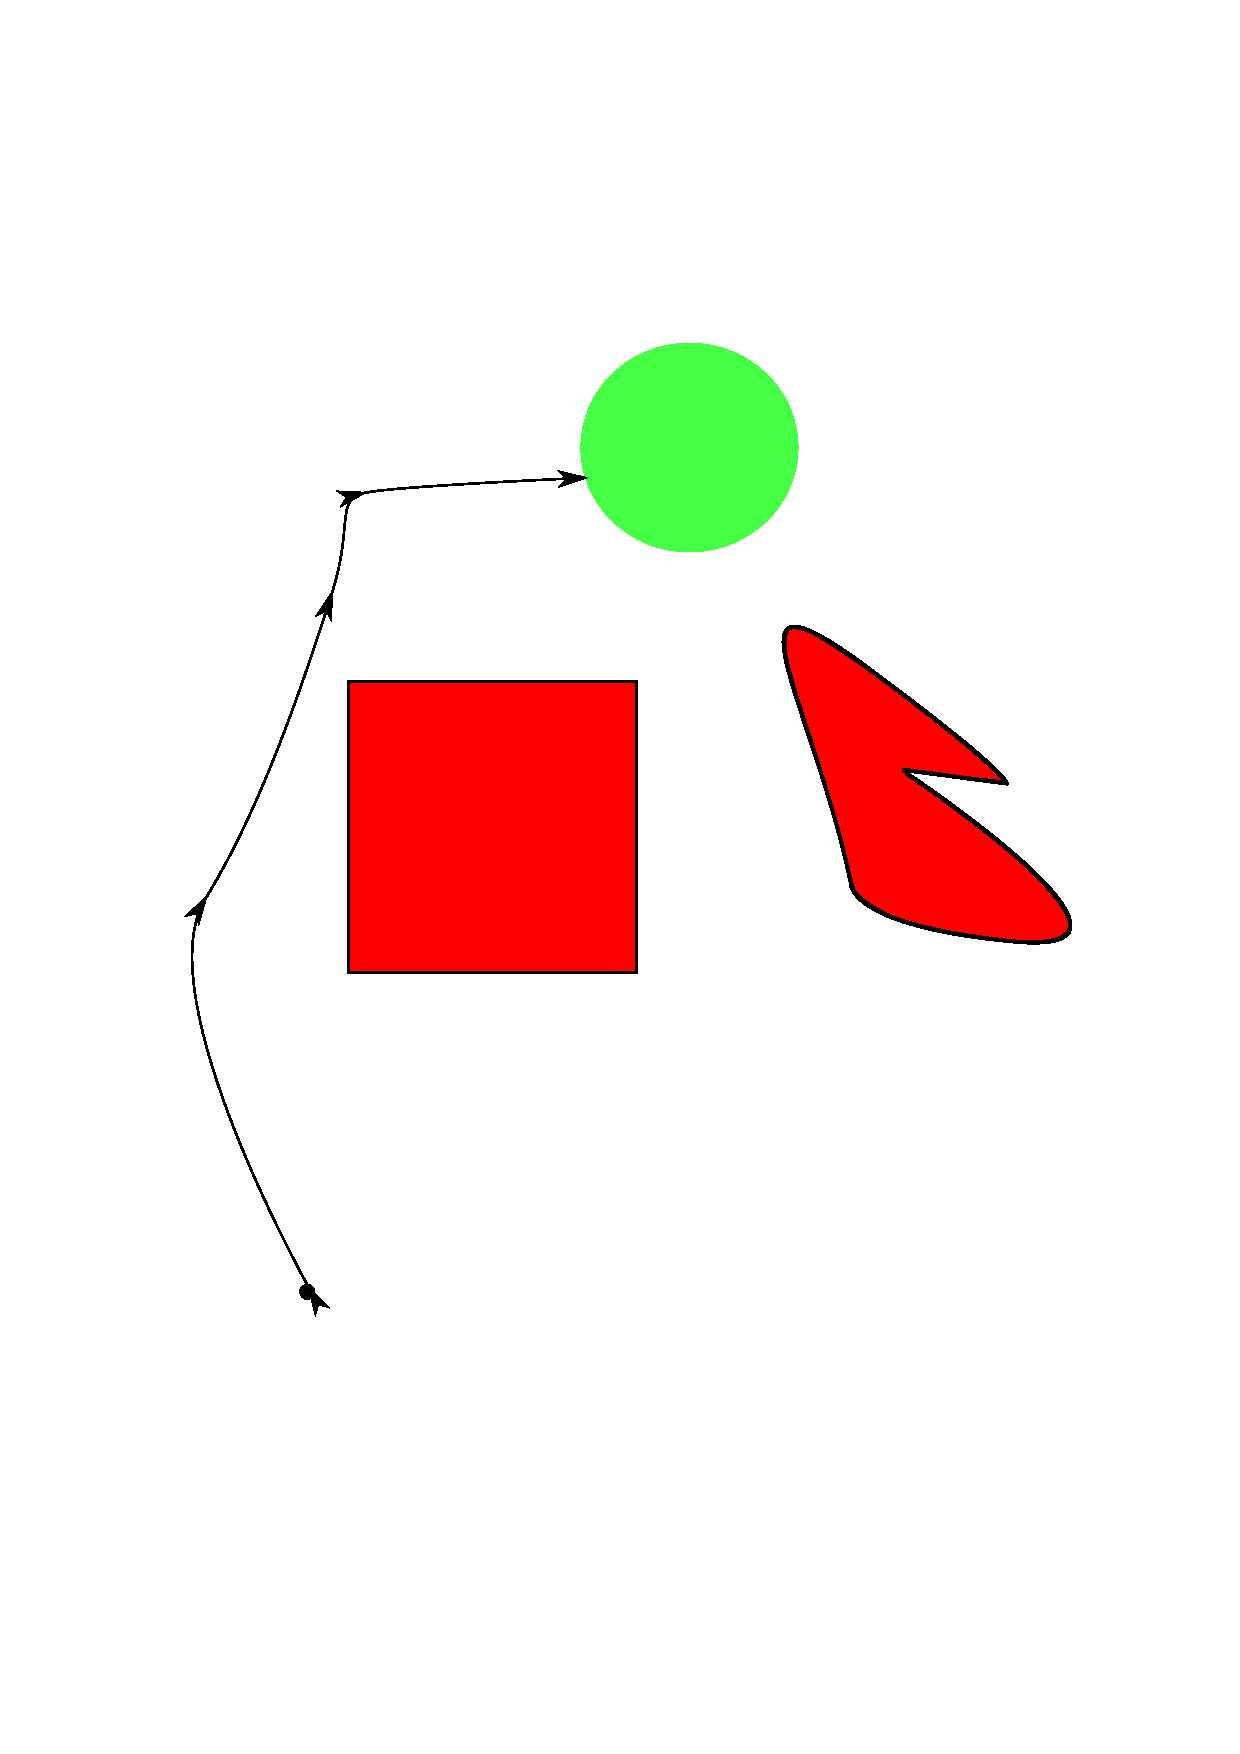
\includegraphics[width=\linewidth]{./Planning/trajectory_3.pdf}
  \end{subfigure}
  \hfill
  \begin{subfigure}[b]{0.24\linewidth}
    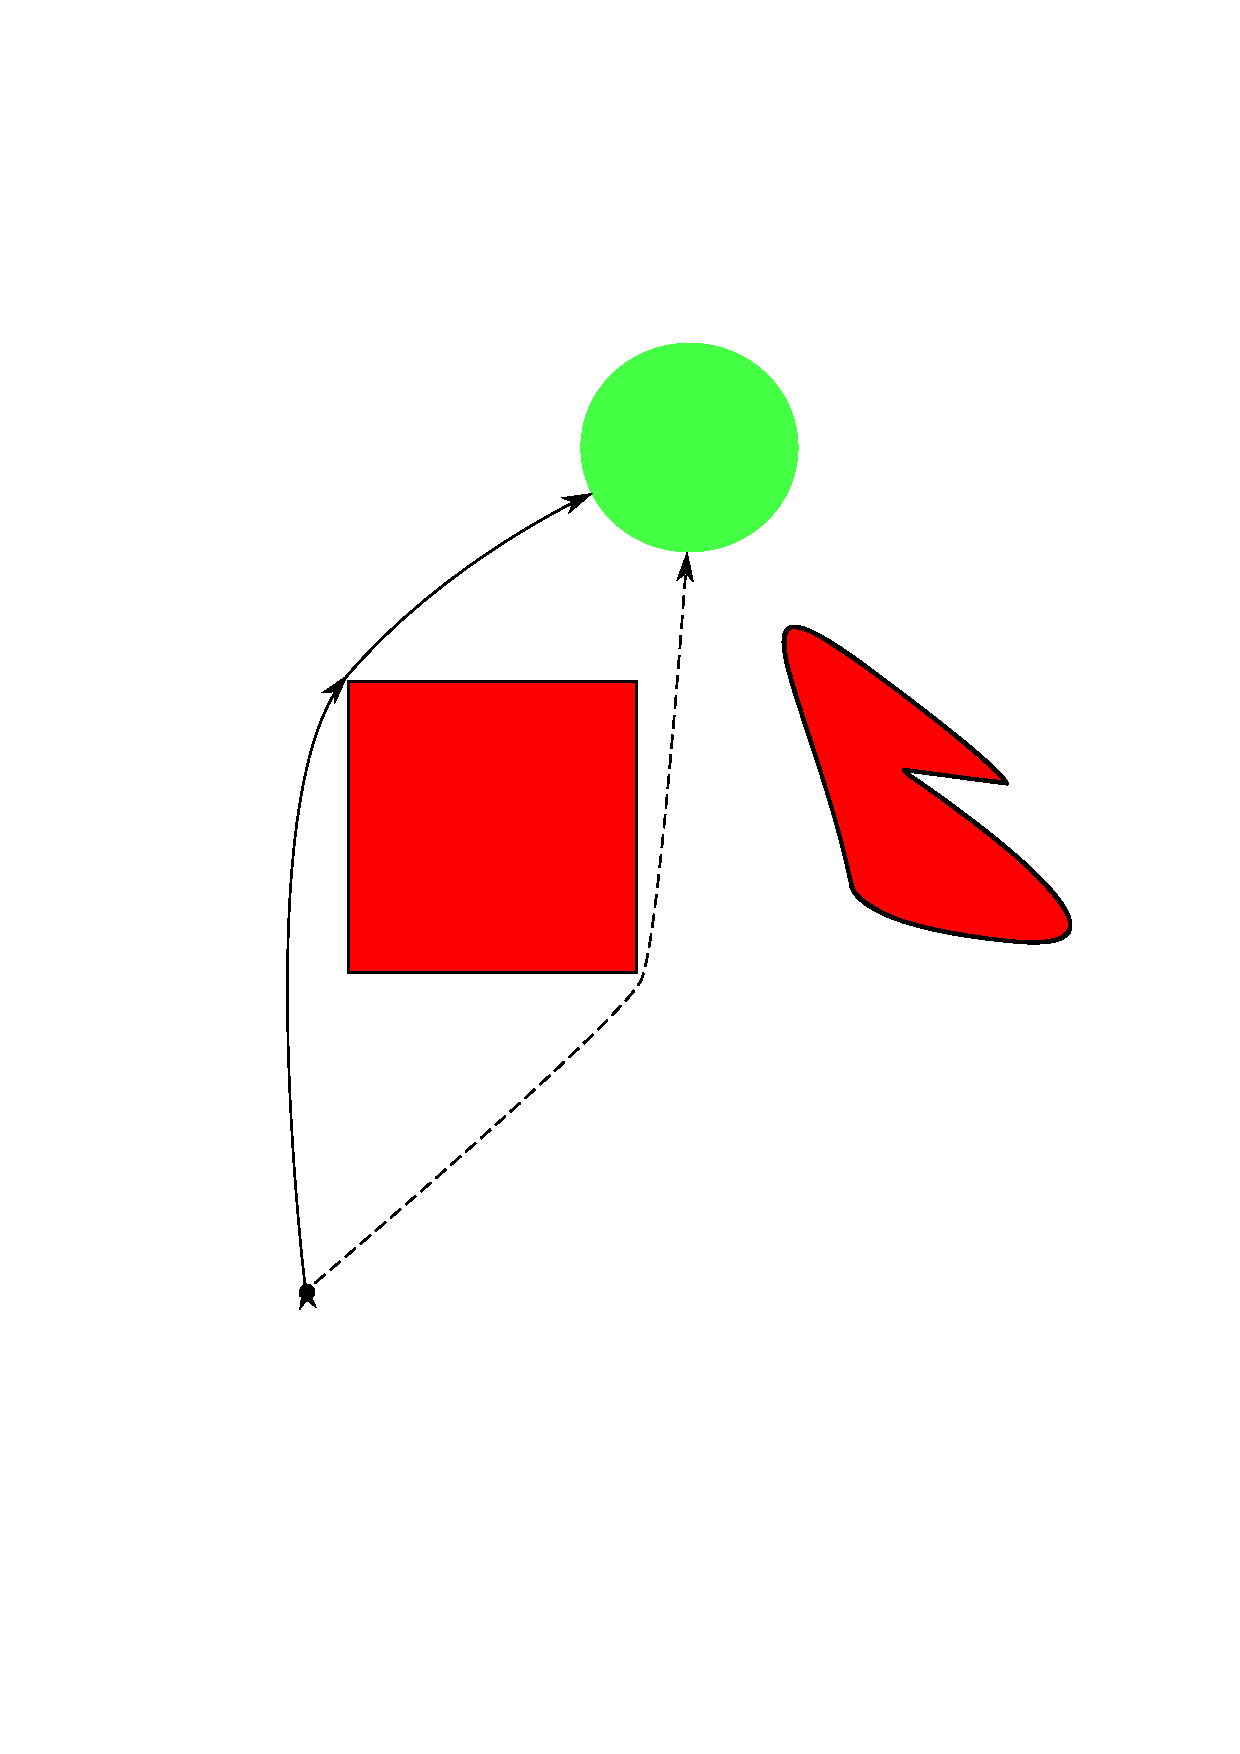
\includegraphics[width=\linewidth]{./Planning/trajectory_best.pdf}    
  \end{subfigure}
  
  \caption{Optimizing the shortest path trajectory from an initial path converges to a local best, but possibly misses the globally best solution.}
  \label{fig:TrajectoryOptimization}
\end{figure}

\subsection{Methods for Finding the Minimum Cost Trajectory}
\subsection{Smoothing the Contacts to Discover Contacts}

Trajectories for a robotic arm are created through trajectory optimization. The key approach used here is softening of contacts through the introduction of auxiliary variables which drastically smooth the cost function used at the expense of increasing the dimensionality of the state space. The formulation used in the paper follows from Mordatch's work \cite{Mordatch2012}.

A trajectory $s$ is a series of robot states $s_t$ at increasing points in time. Each state $s_t$ contains the joint configuration $\theta_t$ as well as an axillary continuous variable $c_t$ for each section of the robotic arm allowed to make contact with the environment. The variables $c_t$ regulate the magnitude of the normal and frictional contact forces and will be describe in detail later in this document. At first these $c$ variables seem unnecessary as the forward kinematics specified by the joint angles $\theta$ determine the locations of the robot, and therefore determine the contacts between the robot and the environment. However slight changes in these joint configurations result in slight motion of the robot which may result in huge changes in contact forces. Additionally without artificial terms in the cost function to model contact, the cost function is blind to potential contacts that may be close and useful. 

\subsubsection{Cost Function}
The optimal solution $s^*$ is computed by minimizing the cost function of the form

\begin{align*}
L(s) &= L_{Contact Violation} + L_{u} \\
&+ L_{Object Penetration} + L_{Goal}   
\end{align*}
    
$L_{Object Penetration}$ and $L_{Goal}$ are straightforward, while the interplay between $L_{Contact Violation}$ and $L_u$ provide the interesting structure allowing the optimization to find paths which use supporting contacts.


\subsubsection{Cost $L_{Contact Violation}$}
Each section of the robot able to make contact has an associated variable $c_t > 0$ at each time step. $c$ intuitively represents the strength of the contact forces. Since if the robot is not physically in contact with the world there will not be a contact force the cost $L_{Contact Violation}$ is introduced to penalize non-zero values of $c$ when the robot is not in contact. 
$$L_{Contact Violation} = \sum_t{\sum_i{c_{t,i} d_{t,i}}}$$
Non-zero values for $c$ are intentionally allowed when the robot is not in contact with the environment even though this is not physically realistic as this makes the cost function smooth. However when optimizing $c_{t,i}$ will tend towards 0 unless the robot is in contact. 

\subsubsection{Cost $L_u$}

The cost $L_u$ penalizes the input torque necessary to follow the trajectory specified. With no contacts these inputs could be calculated directly from the arm inverse dynamics. As discussed the physical contact forces are extremely sensitive to robot configuration, so to soften the forces we instead compute the contact forces that minimize the joint torque. When the trajectory is executed on the robot the joint controller will take responsibility for finding the slight adjustments in configuration to reach the desired contact forces. The path planner does not have to worry about the minute adjustments for a model that will not match reality to that detail anyway. Instead this path planner just needs to estimate the best contact forces possibly, according to the the following quadratic programming problem:
\begin{align*}
f, u &= argmin_{\tilde{f}, \tilde{u}} ||J^T\tilde{f} + \tilde{u} - \tau_{Free}|| \\
&+ \tilde{f}^T W \tilde{f} + \tilde{u}^T R \tilde{u}
\end{align*}

The input control regularization $R$ is chosen based on the desired penalization of joint inputs. The contact force regularization $W$ is dependant on the values of $c$, with 
$$W_{j,j} = \frac{1}{c_{i,t}^2 + 1}$$
If $c$ is large then the robot is in contact, the force regularization is small, so the contact force can be large. If $c$ is small the robot is not near any contact location, the force regularization is large, thus the contact force is heavily penalized and will be small. 


\subsection{Other Cost Terms}
$L_{Obstacle}$ penalizes penetration of the robot into the environment which is calculated using the robot forward kinematics and then collision detection.

$L_{Goal}$ is a penalty on the last robot state $s_T$ on the distance of the robot end effector from the goal location.

\subsubsection{Auxillary Variables}



\section{Sample Based Planning}
\subsection{RRTs and their variants}
\subsection{Adaptation to Encourage Contacts}
Given:
\begin{align*}
    &X \in \mathbb{R}^d:     &&\text{d-dimensional configuration space}\\
    &X_{obs} \subset X:      &&\text{obstacles in the configuration space}\\
    &X_{free} = X \setminus X_{obs}:   &&\text{free space}\\
    &x_{start} \in X_{free}:  &&\text{starting configuration}\\
    &X_{goal} \subset X_{free}: &&\text{set of goal configurations}\\
    &policy: X \times X \rightarrow TX &&\text{policy to goal, maps to tangent space (velocity).  Previous formulation was wrong, as need to be able to follow the policy to an arbitrary point in X, not just a goal configuration}
\end{align*}

The goal is to find a path in $X_{free}$ from $x_{start}$ to $x_{goal} \in X_{goal}$.


\begin{algorithm}
\caption{$T=(V,E) \leftarrow$ policyRRT$(x_{start})$}\label{euclid}
\begin{algorithmic}[1]
\State $T \leftarrow$ InitTree($x_{start}$)
\While {GoalNotReached($T, X_{goal}$)}
\State $x_{rand} \in X \leftarrow$ Sample()
\State $x_{nearest} \leftarrow $ Nearest($T, x_{rand}$)
\State $T \leftarrow $ followPolicy$(x_{nearest}, x_{rand}, T$, extensionLimit)
\If {ExtensionSuccessful}
\State $T \leftarrow $ followPolicy$(x_{new}, x_{goal} \in X_{goal}, T, \infty)$
\EndIf
\EndWhile
\end{algorithmic}
\end{algorithm}

\begin{algorithm}
\caption{$T=(V,E) \leftarrow$ followPolicy$(x_{begin}, x_{end}, T$, iterLimit)}\label{euclid}
\begin{algorithmic}[1]
\State $T_{new} \leftarrow $ InitTree($x_{begin}$)
\State $x_{prev} \leftarrow x_{begin}$
\State $x_{new} \leftarrow $ policy($x_{prev}, x_{end}$)
\State $i \leftarrow 0$
\WhileNoDo{MovingTowardsGoal($x_{new}, T_{new}$) \textbf{and}}
\StatexIndent[2] Nearest($T, x_{new}$) == $x_{begin}$ \textbf{and}
\StatexIndent[2] i $<$ iterLimit
\algorithmicdo
\State $T_{new} \leftarrow $ AddNode($x_{new}, x_{prev}, T_{new}$)
\State $x_{prev} \leftarrow x_{new}$ 
\State $x_{new} \leftarrow $ policy($x_{prev}, x_{end}$)
\State $i \leftarrow i+1$
\EndWhile
\State $T \leftarrow $ AddTreeToTree($T_{new}, T, x_{begin}$)
\end{algorithmic}
\end{algorithm}

In many environments, it is relatively easy to compute a reactive policy that can make forwards progress towards a goal while avoiding collision with obstacles, such as a potential field approach, but such policies are prone to getting stuck in local minima/dead ends.  PolicyRRT is a variant of RRT that seeks to combine the efficient, goal directed trajectory generation of reactive policies with the ability of RRT to find paths around local minima/dead ends.  PolicyRRT fundamentally behaves like a standard RRT by growing a tree by iteratively extending towards a randomly sampled configuration from the nearest point in a search tree $T$.  PolicyRRT uses the reactive policy to move towards the random sample, potentially enabling the planner to avoid collisions with obstacles during the extension.  When PolicyRRT is successful in extending towards the sample (does not collide with an obstacle and does not get stuck in a local minima) it then follows the policy to extend towards the goal.  To avoid oversampling regions associated with local minima, when PolicyRRT extends towards a point from some vertex $v \in T$ PolicyRRT halts extension when the trajectory leaves the Voronoi cell of $v$.  Extension is also halted once the policy ceases to make progress (reaches a local minima) or exceeds a maximum number of iterations (only when extending towards $x_{rand}$?)

PolicyRRT is beneficial when a policy that would yield a path all the way from $x_{start}$ and $x_{goal}$ is difficult to find but finding a policy that can make some progress while avoiding obstacles, but may get stuck in local minima is relatively easy. An example of such a policy is a \textbf{potential field}: a cost function is constructed by placing attractors at the goals and repulsions at obstacles and the policy is to the gradient of this cost.  Potential fields are generally much simpler to compute than the minima-free navigation functions, but cannot be guaranteed to produce a path.  Augmenting the gradient descent policy with an RRT can help find paths out of any local minima.

Similarly augmenting an RRT with a reactive policy can assist in navigating narrow passages.  Because the policy will naturally flow through corridors PolicyRRT no longer requires drawing samples inside the narrow corridor itself, as drawing a sample from the far side may suffice to draw the policy through the corridor.

\begin{figure}
  \centering
  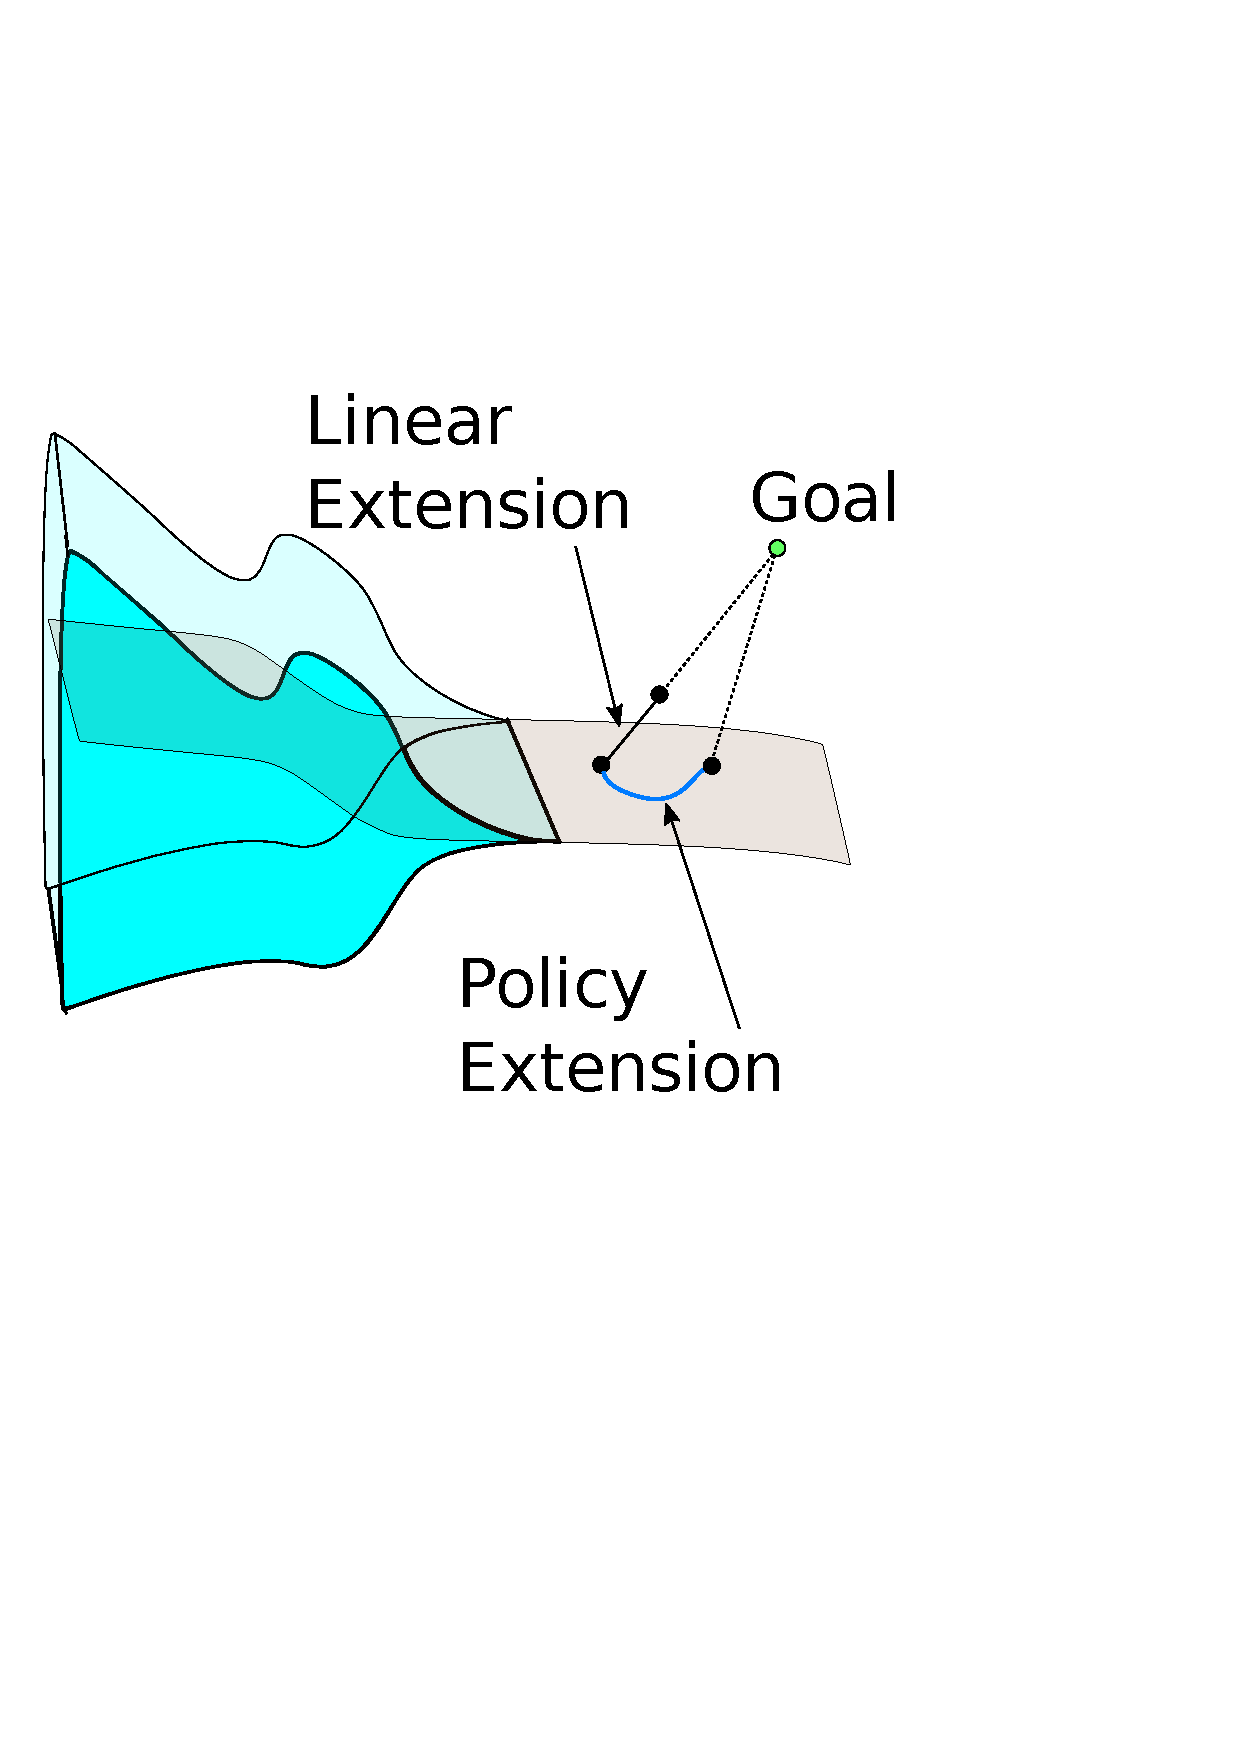
\includegraphics[width=.5\linewidth]{./Planning/extend.pdf}
  
  \caption{Illustration of Gradient RRT extension on the contact manifold}
  \label{fig:Extend}
\end{figure}


\section{Experiments}
\subsection{Simulation and Robot Model}
\subsection{Robot Snakes on a Plane}

\end{document}
